\documentclass[border=3pt]{standalone}
% Preâmbulo compartilhado pelos diagramas TikZ da aula 4 de Navegação (Representação de Mapas)
\usepackage[T1]{fontenc}
\usepackage[utf8]{inputenc}
\usepackage{lmodern}
\usepackage{amsmath}
\usepackage{xcolor}
\usepackage{tikz}
\usetikzlibrary{arrows.meta,angles,quotes,decorations.pathmorphing,decorations.pathreplacing,calc,
                positioning,shapes.geometric,shapes.misc,backgrounds,fit,
                math}

% Paleta (mesma dos SVGs originais)
\definecolor{dblue}{HTML}{2A5B8C}
\definecolor{dorange}{HTML}{B3541E}
\definecolor{dgreen}{HTML}{4A7C59}
\definecolor{dred}{HTML}{9C4B4B}
\definecolor{dcream}{HTML}{F4F1EA}
\definecolor{dshade}{HTML}{DDD7C9}

% Função gaussiana (não normalizada por padrão de escala visual)
\pgfmathdeclarefunction{gauss}{3}{%
  \pgfmathparse{1/(#3*sqrt(2*pi))*exp(-((#1-#2)^2)/(2*#3^2))}%
}

% Estilos comuns (prefixo d... para não colidir com chaves internas do pgf)
\tikzset{
  >={Stealth[length=2mm]},
  dguide/.style={gray!55, dashed, line width=0.4pt},
  daxis/.style={gray!60, line width=0.7pt, ->},
  dbody/.style={fill=black!3, draw=black!80, line width=1pt},
  dacc/.style={draw=dblue, line width=1pt},
  dlbl/.style={black!55, font=\small},
  dsub/.style={black!45, font=\footnotesize},
  dstate/.style={circle, draw=black!80, fill=dcream, line width=1pt,
                 minimum size=17mm, font=\large, inner sep=1pt},
  dobs/.style={circle, draw=black!80, fill=dshade, line width=1pt,
               minimum size=14mm, font=\large, inner sep=1pt},
  dbox/.style={rounded corners=2pt, draw=black!80, fill=dcream, line width=1pt,
               align=center, inner sep=6pt},
  dop/.style={circle, draw=black!80, fill=white, line width=1pt,
              minimum size=6mm, inner sep=0pt, font=\small},
  dtrans/.style={->, dblue, line width=1pt},
  dmeas/.style={->, dorange, line width=1pt},
  dcurve/.style={line width=1pt, dblue},
  dcurveb/.style={line width=1.4pt, dorange},
}

\begin{document}
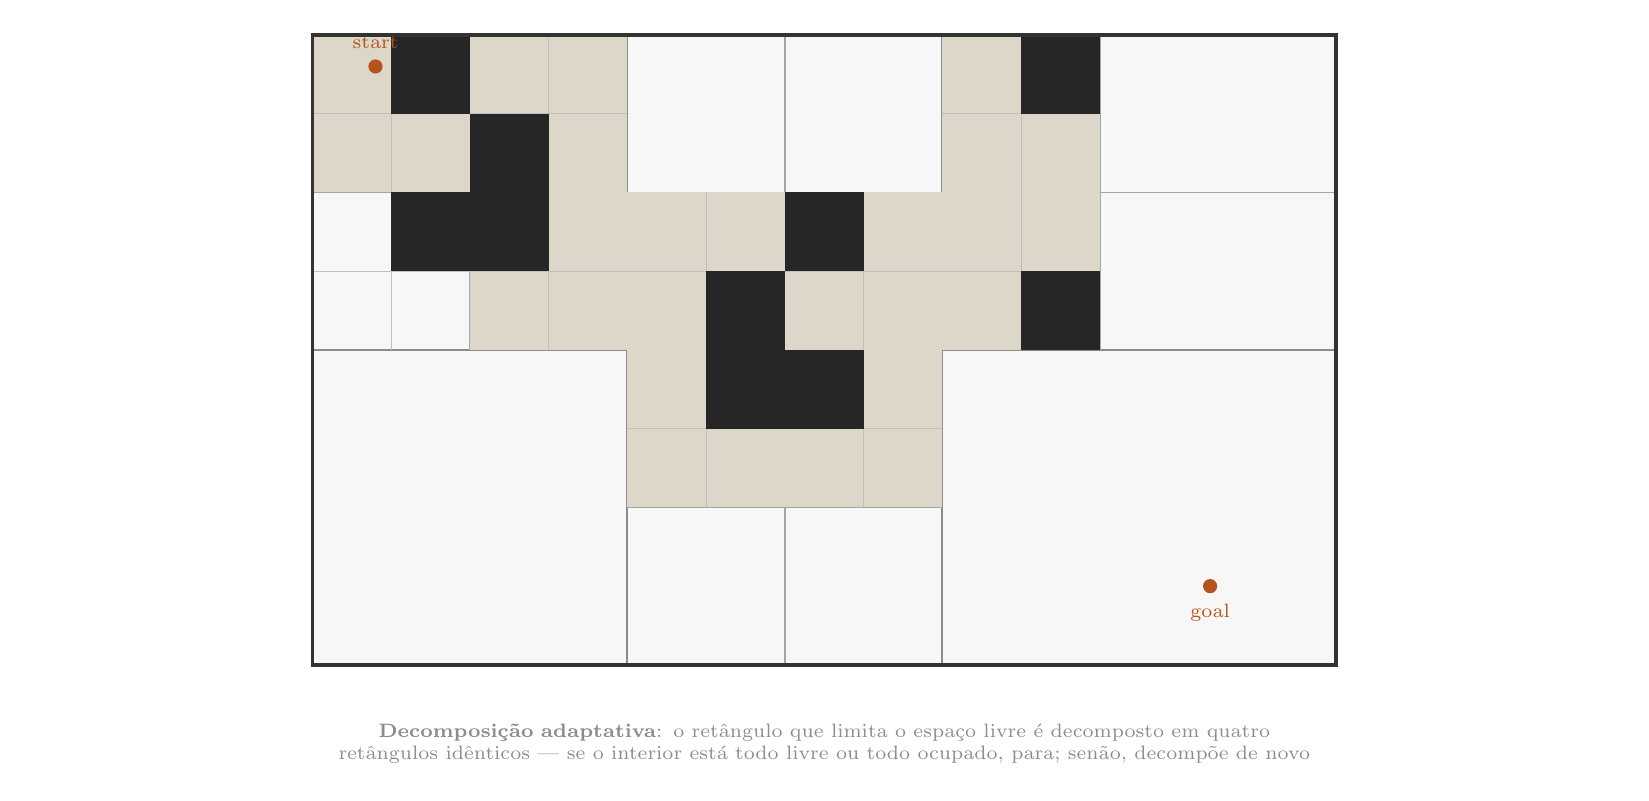
\begin{tikzpicture}[x=1cm,y=1cm]

  \draw[dbody, line width=1.2pt] (0,0) rectangle (13,8);

  % Nível 1: divide em 6 blocos grandes
  \draw[black!45, line width=0.7pt] (4,0) -- (4,8);
  \draw[black!45, line width=0.7pt] (8,0) -- (8,8);
  \draw[black!45, line width=0.7pt] (0,4) -- (13,4);

  % ---- Bloco livre grande: [0,4]x[0,4] --- não subdivide ----
  % ---- Bloco livre grande: [8,13]x[0,4] --- não subdivide ----

  % ---- Bloco [0,4]x[4,8]: contém o obstáculo A (dardo) ----
  \draw[black!35, line width=0.5pt] (2,4) -- (2,8);
  \draw[black!35, line width=0.5pt] (0,6) -- (4,6);
  \fill[dshade] (0,6) rectangle (2,8);
  \fill[dshade] (2,6) rectangle (4,8);
  \draw[black!25, line width=0.35pt] (1,6) -- (1,8);
  \draw[black!25, line width=0.35pt] (0,7) -- (2,7);
  \fill[black!85] (1,7) rectangle (2,8);
  \draw[black!25, line width=0.35pt] (3,6) -- (3,8);
  \draw[black!25, line width=0.35pt] (2,7) -- (4,7);
  \fill[black!85] (2,6) rectangle (3,7);
  \draw[black!25, line width=0.35pt] (1,4) -- (1,6);
  \draw[black!25, line width=0.35pt] (0,5) -- (2,5);
  \fill[black!85] (1,5) rectangle (2,6);
  \fill[dshade] (2,4) rectangle (4,6);
  \draw[black!25, line width=0.35pt] (3,4) -- (3,6);
  \draw[black!25, line width=0.35pt] (2,5) -- (4,5);
  \fill[black!85] (2,5) rectangle (3,6);

  % ---- Bloco [4,8]x[4,8]: contém topo do obstáculo B (pentágono) ----
  \draw[black!35, line width=0.5pt] (6,4) -- (6,8);
  \draw[black!35, line width=0.5pt] (4,6) -- (8,6);
  \fill[dshade] (4,4) rectangle (6,6);
  \draw[black!25, line width=0.35pt] (5,4) -- (5,6);
  \draw[black!25, line width=0.35pt] (4,5) -- (6,5);
  \fill[black!85] (5,4) rectangle (6,5);
  \fill[dshade] (6,4) rectangle (8,6);
  \draw[black!25, line width=0.35pt] (7,4) -- (7,6);
  \draw[black!25, line width=0.35pt] (6,5) -- (8,5);
  \fill[black!85] (6,5) rectangle (7,6);

  % ---- Bloco [8,13]x[4,8]: contém o obstáculo C (triângulo) ----
  \draw[black!35, line width=0.5pt] (10,4) -- (10,8);
  \draw[black!35, line width=0.5pt] (8,6) -- (13,6);
  \fill[dshade] (8,6) rectangle (10,8);
  \draw[black!25, line width=0.35pt] (9,6) -- (9,8);
  \draw[black!25, line width=0.35pt] (8,7) -- (10,7);
  \fill[black!85] (9,7) rectangle (10,8);
  \fill[dshade] (8,4) rectangle (10,6);
  \draw[black!25, line width=0.35pt] (9,4) -- (9,6);
  \draw[black!25, line width=0.35pt] (8,5) -- (10,5);
  \fill[black!85] (9,4) rectangle (10,5);

  % ---- Bloco [4,8]x[0,4]: contém a base do obstáculo B ----
  \draw[black!35, line width=0.5pt] (6,0) -- (6,4);
  \draw[black!35, line width=0.5pt] (4,2) -- (8,2);
  \fill[dshade] (4,2) rectangle (6,4);
  \draw[black!25, line width=0.35pt] (5,2) -- (5,4);
  \draw[black!25, line width=0.35pt] (4,3) -- (6,3);
  \fill[black!85] (5,3) rectangle (6,4);
  \fill[dshade] (6,2) rectangle (8,4);
  \draw[black!25, line width=0.35pt] (7,2) -- (7,4);
  \draw[black!25, line width=0.35pt] (6,3) -- (8,3);
  \fill[black!85] (6,3) rectangle (7,4);

  \draw[draw=black!80, line width=1.2pt] (0,0) rectangle (13,8);

  \fill[dorange] (0.8,7.6) circle (0.09);
  \node[dorange, font=\scriptsize, anchor=south] at (0.8,7.7) {start};
  \fill[dorange] (11.4,1.0) circle (0.09);
  \node[dorange, font=\scriptsize, anchor=north] at (11.4,0.9) {goal};

  \node[dsub, font=\scriptsize, align=center, text width=20cm] at (6.5,-1.0)
     {\textbf{Decomposição adaptativa}: o retângulo que limita o espaço livre é decomposto em quatro retângulos idênticos --- se o interior está todo livre ou todo ocupado, para; senão, decompõe de novo};

\end{tikzpicture}
\end{document}
